\documentclass[11pt]{article}
\usepackage{ucs}
\usepackage[utf8x]{inputenc}
\usepackage{changepage}
\usepackage{graphicx}
\usepackage{amsmath}
\usepackage{gensymb}
\usepackage{amssymb}
\usepackage{enumerate}
\usepackage{tabularx}
\usepackage{lipsum}
\usepackage{amsthm}
\usepackage{thmtools}


\usepackage{fontspec} % loaded by polyglossia, but included here for transparency 
\usepackage{polyglossia}

\usepackage{xeCJK}
\setCJKmainfont{SimSun}
\setmainlanguage{russian} 
\setotherlanguage{english}

\newfontfamily\cyrillicfont[Script=Cyrillic]{Times New Roman}
\newfontfamily\cyrillicfontsf[Script=Cyrillic]{Arial}
\newfontfamily\cyrillicfonttt[Script=Cyrillic]{Courier New}

\oddsidemargin 0.0in
\evensidemargin 0.0in
\textwidth 6.27in
\headheight 1.0in
\topmargin 0.0in
\headheight 0.0in
\headsep 0.0in
%\textheight 9.69in
\textheight 9.00in
 
\setlength\parindent{0pt}

\newenvironment{myenv}{\begin{adjustwidth}{0.4in}{0.4in}}{\end{adjustwidth}}
\renewcommand{\abstractname}{Anotācija}
\renewcommand\refname{Atsauces}

%\newenvironment{uzdevums}[1][\unskip]{%
%\vspace{3mm}
%\noindent
%\textbf{#1:}
%\noindent}
%{}

% (4;10;12;17)
% (p1.19;5;15;20)

% http://tex.stackexchange.com/questions/196961/thmtools-declaration-for-theorem-and-proof
\declaretheoremstyle[headfont=\normalfont\bfseries,notefont=\mdseries\bfseries,bodyfont = \normalfont,headpunct={:}]{normalhead}
\declaretheorem[name={Uzdevums}, style=normalhead,numberwithin=section]{problem}

%\def\changemargin#1#2{\list{}{\rightmargin#2\leftmargin#1}\item[]}
\def\changemargin#1#2{\list{}\item[]}
\let\endchangemargin=\endlist 


\newcommand{\subf}[2]{%
  {\small\begin{tabular}[t]{@{}c@{}}
  #1\\#2
  \end{tabular}}%
}



\newcounter{alphnum}
\newenvironment{alphlist}{\begin{list}{(\Alph{alphnum})}{\usecounter{alphnum}\setlength{\leftmargin}{2.5em}} \rm}{\end{list}}

\newenvironment{zhtext}{\fontfamily{MS PGothic}\selectfont}{\par}


\makeatletter
\let\saved@bibitem\@bibitem
\makeatother

\usepackage{bibentry}
%\usepackage{hyperref}

\newenvironment{tulkojums}[1][\unskip]{%
\begin{changemargin}{8mm}{8mm}
\fontsize{9}{11}
\selectfont
\textbf{#1:}
}
{ 
\fontsize{12}{14}
\selectfont
\end{changemargin}
}

\setcounter{section}{1}


\begin{document}

\begin{center}
{\Large \bf 7.-9.kl. uzdevumi ar matemātiskās indukcijas elementiem}
\end{center}

\begin{problem}[EE.PK.1993.9.5]
Rindā izvietotas $n$ ārēji atšķirīgas figūriņas. 
Ir atļauts mainīt vietām jebkuras divas figūriņas, 
starp kurām atrodas tieši viena cita figūriņa. 
Vai ar šādiem pārvietojumiem var visas figūriņas pārlikt
secībā, kura ir pretēja sākotnējai? Pamatot atbildi. 
\end{problem}



\begin{problem}[EE.PK.1994.9.1]
Atrast koeficientu $a_{50}$ šādā identitātē:
$$\left( 1 + x + \ldots + x^{100} \right) \left( 1 + x + \ldots + x^{25} \right)
= 1 + a_1x + \ldots + a_{125}x^{125}.$$
\end{problem}




\begin{problem}[EE.PK.1995.7.3]
Kādā 20-stāvu ēkā lifts sabojāts tādā veidā, ka ar to var 
uzbraukt vai nu 8 stāvus uz augšu, vai arī 11 stāvus uz leju
(ja uz augšu vai uz leju nav tik daudz stāvu, tad attiecīgajā virzienā 
lifts nepārvietojas). 
\begin{enumerate}[(a)]
\item Vai ar liftu var no 20. stāva nobraukt uz pirmo?
\item Uz kuriem stāviem var ar šo liftu aizbraukt no pirmā stāva?
\end{enumerate}
({\em Sk. arī LV.AO.2013.5.2.})
\end{problem}


\begin{problem}[EE.PK.1998.7.TEST.5]
Skaitļi izkārtoti rindās tā, kā parādīts zīmējumā. 
Kāds skaitlis atrodas devītās rindas vidū?
\begin{center}
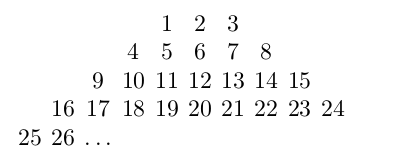
\includegraphics[width=0.4\textwidth]{math-induction-junior-classes/EE-PK-1998-7-TEST-4.png}
\end{center}
\end{problem}

\begin{problem}[EE.PK.2001.8.TEST.5]
Naturālie skaitļi, sākot no $1$, izvietoti 
trijstūrveida tabulā, kuras pirmās četras rindas redzamas zīmējumā. 
Par cik skaitlis, kurš 17.rindā ir pirmais no kreisās, 
ir mazāks par to skaitli, kurš 19.rindā ir pirmais no labās?
\begin{center}
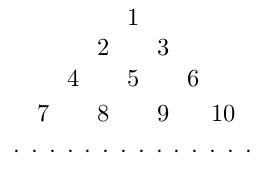
\includegraphics[width=0.25\textwidth]{math-induction-junior-classes/EE-PK-2001-8-TEST-5.png}
\end{center}
\end{problem}



\begin{problem}[EE.PK.2001.8.TEST.5]
Naturālos skaitļus no $1$ līdz $2001$ raksta tabulā, kura 
sastāv no septiņām kolonnām, kā attēlots zīmējumā. 
Ar kādu burtu apzīmēta kolonna, kurā ierakstīs skaitli $2001$?
\begin{center}
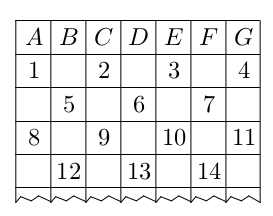
\includegraphics[width=0.25\textwidth]{math-induction-junior-classes/EE-PK-2001-9-TEST-5.png}
\end{center}
\end{problem}

\begin{problem}[EE.PK.2003.9.4]
Zīmējumā attēlota dzelzceļa mezgla shēma. No kreisās puses uz 
labo tam tuvojas $8$ lokomotīves, kuras var virzīties pa 
šo ceļu tikai no kreisās uz labo pusi. 
Parādīt, kā var pārkārtot lokomotīves šajā dzelzceļa mezglā tā, lai 
tās labajā pusē izbrauktu secībā, kas ir pretēja sākotnējai. 
(Katrs ceļa posms šajā mezglā ir pietiekami garš, lai vajadzības 
gadījumā tur novietotos visas lokomotīves.)
\begin{center}
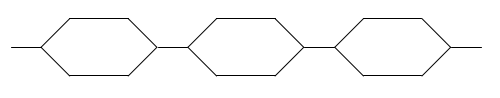
\includegraphics[width=0.4\textwidth]{math-induction-junior-classes/EE-PK-2003-9-4.png}
\end{center}
\end{problem}

\begin{problem}[EE.PK.2004.9.4]
Marija un Juris spēlē sekojošu spēli uz laukuma, 
ko veido $n$ rūtiņu virkne ($n > 2$). 
Katram spēlētājam ir viena figūriņa, abas figūriņas 
spēles sākumā novietotas spēles laukuma abos galos. 
Vienā gājienā spēlētājs pārvieto savu figūriņu par vienu vai 
divām rūtiņām jebkurā virzienā. 
Uzvar tas spēlētājs, kurš novieto savu figūriņu uz tās
rūtiņas, kurā atrodas pretinieka figūriņa. 
Kādām $n$ vērtībām Marijai ir uzvaroša stratēģija; 
pie kādām $n$ vērtībām Jurim ir uzvaroša stratēģija.
\end{problem}

\begin{problem}[EE.PK.2005.9.4]
Doti $2005$ veseli skaitļi. Burvis Merlins spēlē šādu spēli. 
Vienā gājienā viņš izvēlas $7$ skaitļus, un katru izvēlēto 
skaitli (neatkarīgi no citiem izvēlētajiem) palielina par $1$
vai reizina ar $-1$. Pierādīt, ka pēc galīga gājienu skaita 
Merlins var visus $2005$ skaitļus pārvērst par nullēm. 
\end{problem}

\begin{problem}[EE.PK.2006.9.TEST.4]
Atrast izteiksmes vērtību:
$$1 + \frac{100}{2006} - \frac{101}{2006} + \frac{102}{2006} - \frac{103}{2006} + \ldots,$$
ja izteiksme satur $1003$ zīmes ``$+$'' un $1003$ zīmes ``$-$''.
\end{problem}

\begin{problem}[EE.PK.2006.9.4]
Katrs Brīnumzemes iedzīvotājs vai nu vienmēr runā patiesību, vai 
arī vienmēr melo. Reiz visus Brīnumzemes iedzīvotājus sadalīja
pa pāriem un katrs no viņiem pateica par savu pāra kaimiņu 
"Viņš melo" vai arī "Viņš saka patiesību". Vai varēja gadīties, 
ka abi šie apgalvojumi tika izteikti vienādu skaitu reižu, ja 
Brīnumzemē ir {\bf (a)} $2004$ iedzīvotāji?\\
{\bf (b)} $2006$ iedzīvotāji?
\end{problem}


\begin{problem}[EE.PK.2007.7.TEST.6]
Cik dažādos veidos var izveidot skaitli $2007$, sākot ar 
zīmējumā attēloto trijstūrīti, kurā ir cipars $2$ un 
katrā solī pārvietojoties no viena trijstūrīša uz citu, 
kuram ar iepriekšējo ir kopīga mala?
\begin{center}
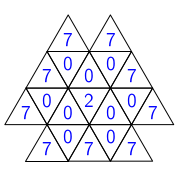
\includegraphics[width=0.2\textwidth]{math-induction-junior-classes/EE-PK-2007-7-TEST-6.png}
\end{center}
\end{problem}


\begin{problem}[EE.PK.2007.8.TEST.6]
Cik dažādos veidos var izveidot skaitli $2007$, ja 
zīmējumā redzamajā figūrā sāk ar aplīti, kurā ir cipars $2$ un 
katrā solī pārvietojas uz citu aplīti, kas pieskaras iepriekšējam? 
\begin{center}
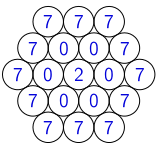
\includegraphics[width=0.2\textwidth]{math-induction-junior-classes/EE-PK-2007-8-TEST-6.png}
\end{center}
\end{problem}


\begin{problem}[EE.PK.2007.9.TEST.6]
Cik dažādos veidos var izveidot skaitli $2007$, sākot ar kvadrātiņu, kurā 
ir skaitlis $2$ un katrā solī pārvietojoties uz citu kvadrātu, kuram ar iepriekšējo ir 
kopīga mala vai kopīga virsotne?
\begin{center}
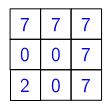
\includegraphics[width=0.15\textwidth]{math-induction-junior-classes/EE-PK-2007-9-TEST-6.png}
\end{center}
\end{problem}

\begin{problem}[EE.PK.2008.9.3]
Rūtiņu laukumā $8 \times 8$ daļa no rūtiņām iekrāsotas 
melnas, bet pārējās \textendash{} baltas. Katrā solī izvēlas
vienu rūtiņu; tad taisnstūrī, kura kreisais augšējais stūris ir 
visa $8 \times 8$ laukuma stūris, bet labais apakšējais stūris 
ir izraudzītā rūtiņa, nomaina visu rūtiņu krāsojumu uz pretējo. 
Vai ar šādiem soļiem no jebkura sākotnējā krāsojuma var sasniegt
stāvokli, kurā visas rūtiņas ir baltas?
\end{problem}


\begin{problem}[EE.PK.2011.7.TEST.10]
Marija salikusi uz galda kaudzīti ar $20$ mandarīniem trijstūra 
piramīdas veidā. Pirmos $10$ mandarīnus viņa liek uz galda tā, 
kā parādīts kreisajā zīmējumā, virs tiem viņa liek slāni no $6$ 
mandarīniem (katrs no kuriem balstās uz trim mandarīniem no zemāk
esošā slāņa), un tā tālāk. 
\begin{center}
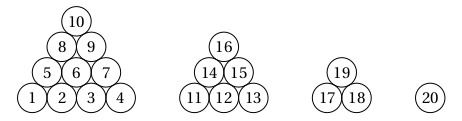
\includegraphics[width=0.6\textwidth]{math-induction-junior-classes/EE-PK-2011-7-TEST-10.png}
\end{center}
Mandarīnus var no kaudzītes paņemt pa vienam. Bet nevar paņemt mandarīnu, kurš
pieskaras tādam mandarīnam, kurš atrodas augstāk. Kāds mazākais skaits mandarīnu 
no kaudzītes jāpaņem, pirms radīsies iespēja dabūt mandarīnu 
{\bf (a)} ar numuru $6$? 
{\bf (b)} ar numuru $4$? 
{\bf (c)} ar numuru $7$?
\end{problem}


\begin{problem}[EE.PK.2011.9.3]
Skaitļiem $x$ un $y$ pieraksts $x \ast y$ apzīmē skaitli 
${\displaystyle \frac{x+y}{xy+4}}$. Atrast izteiksmes vērtību:
$$0 \ast \left(  1 \ast \left( 2 \ast \left( 3 \ast \left(  
4 \ast \left( 5 \ast \left(  6 \ast \left( 
7 \ast \left( 8 \ast 9 \right)
\right) \right) \right)
\right) \right) \right) \right)$$
\end{problem}


\begin{problem}[EE.PK.2017.7.1]
Virknē uzrakstīti $7$ naturāli skaitļi, no kuriem pirmais 
ir $a$ un ir $b$. Katrs nākamais skaitlis šajā virknē vienāds 
ar divu to virknes skaitļu summu, kuri uzrakstīti tieši pirms viņa.\\
{\bf (a)} Atrast pēdējo skaitli šajā virknē, izsakot to ar $a$ un $b$.\\
{\bf (b)} Atrast lielāko iespējamo skaitļa $a$ vērtību, ja zināms, 
ka pēdējais skaitlis virknē ir $2017$.
\end{problem}


\begin{problem}[EE.PK.2017.9.4]
Uz rūtiņu laukuma $8 \times 8$ daļa rūtiņu nokrāsotas baltas, 
bet pārējās melnas. Vienā gājienā var izvēlēties jebkuru 
taisnstūri ar izmēru $2 \times 3$ vai $3 \times 2$, kura 
malas sakrīt ar rūtiņu līnijām, un pārkrāsot visas melnās rūtiņas
baltas un visas baltās rūtiņas melnas. Vai jebkuram sākotnējam krāsojumam 
ar minētajiem gājieniem var iegūt tādu laukumu, kurā 
visas rūtiņas ir melnas?
\end{problem}

\end{document}





